\addcontentsline{toc}{chapter}{MAVEN}
\chapter*{MAVEN}
\stepcounter{chapter}
%Aqui usaremos paradigma de micro servicio en nuestro caso api rest
\section{MVN}
Apache Maven es una herramienta de comprensión y gestión de proyectos de software. Basado en el concepto de un modelo de objetos de proyecto (POM), Maven puede administrar la construcción, los informes y la documentación de un proyecto desde una pieza central de información. Se descarga de la siguiente dirección  \url{https://maven.apache.org/download.cgi}, se instala y se verifica como sigue
\begin{verbatim}
tomas@debian:~$ mvn --version
Apache Maven 3.6.3
Maven home: /usr/share/maven
Java version: 17.0.4, vendor: Debian, runtime: /usr/lib/jvm/java-17-openjdk-amd64
Default locale: en_GB, platform encoding: UTF-8
OS name: "linux", version: "5.10.0-19-amd64", arch: "amd64", family: "unix"
\end{verbatim}
\begin{figure}[h]
\centering
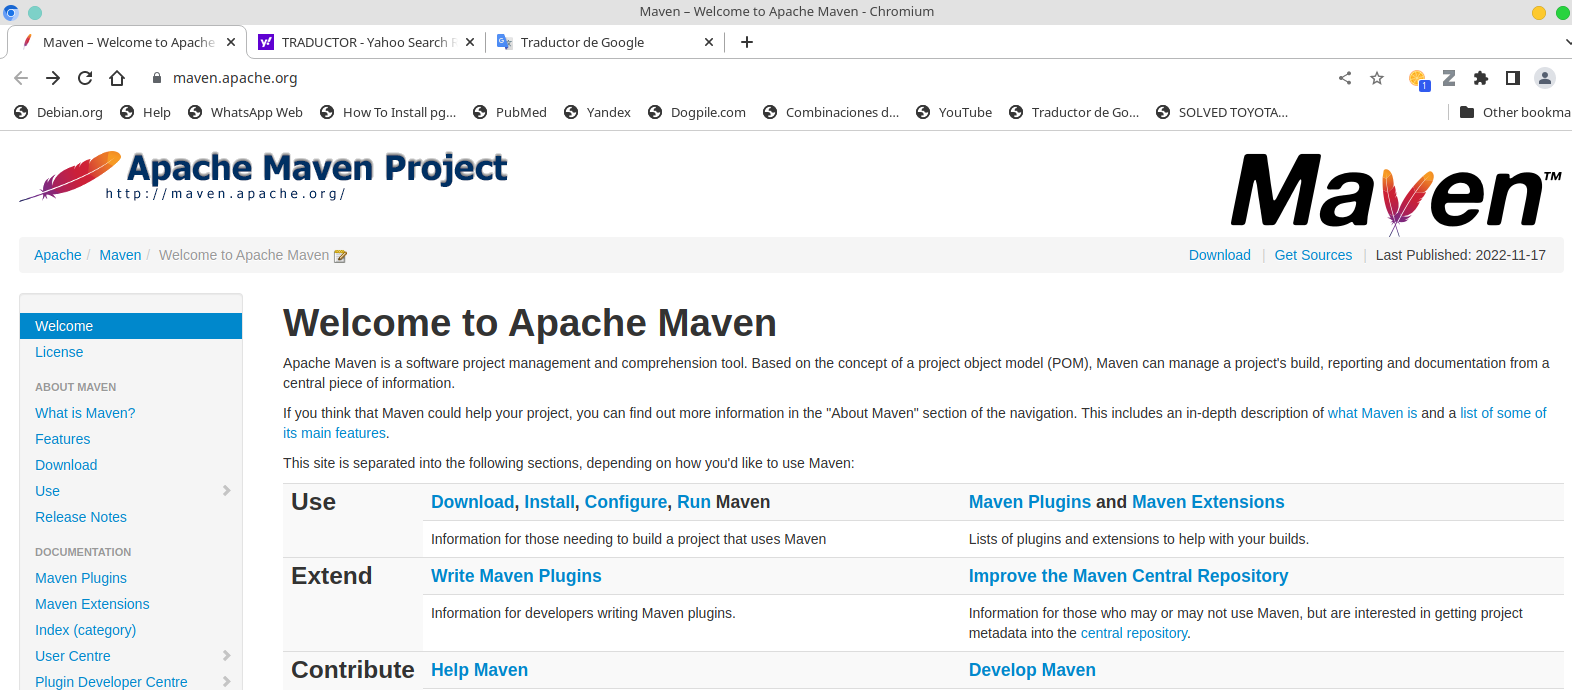
\includegraphics[scale=0.4]{images/maven1}
\caption{Página principal de maven}
\end{figure}
Se debe descara el binario comprimido en .tar (tape archiv); en window se puede descargar lo que puedes descomprimir (generalmente .zip). En windows se descomprime y se configura la carpeta binaria en los variable de entorno. 
\subsection{PROJECT OBJECT MODEL (POM)}
Es un xml  que contiene información a cerca del proyecto y configuración usado por Maven para compilar el proyecto. Project Object Model o POM es la parte básica de la funcionalidad de Maven. Este es un archivo XML que tiene información sobre las dependencias, configuraciones y otra información importante sobre el proyecto. Maven revisa esta información y luego realiza la tarea designada.

Spring Initializr es una API \footnote{ interfaz de programación de aplicaciones API es una forma en que dos o más programas de computadora se comunican entre sí. Es un tipo de interfaz de software que ofrece un servicio a otras piezas de software} que permite la generación de proyectos con sus dependencias permitiendo simplificar esta etapa inicial de arranque de nuevos proyectos. 